%-------------------------------------------------------------------------------
%-------------------------------------------------------------------------------
\section{Network inference: a brief introduction}
%-------------------------------------------------------------------------------
%-------------------------------------------------------------------------------

%-------------------------------------------------------------------------------
\frame{ \frametitle{Typical aim}

  $$
  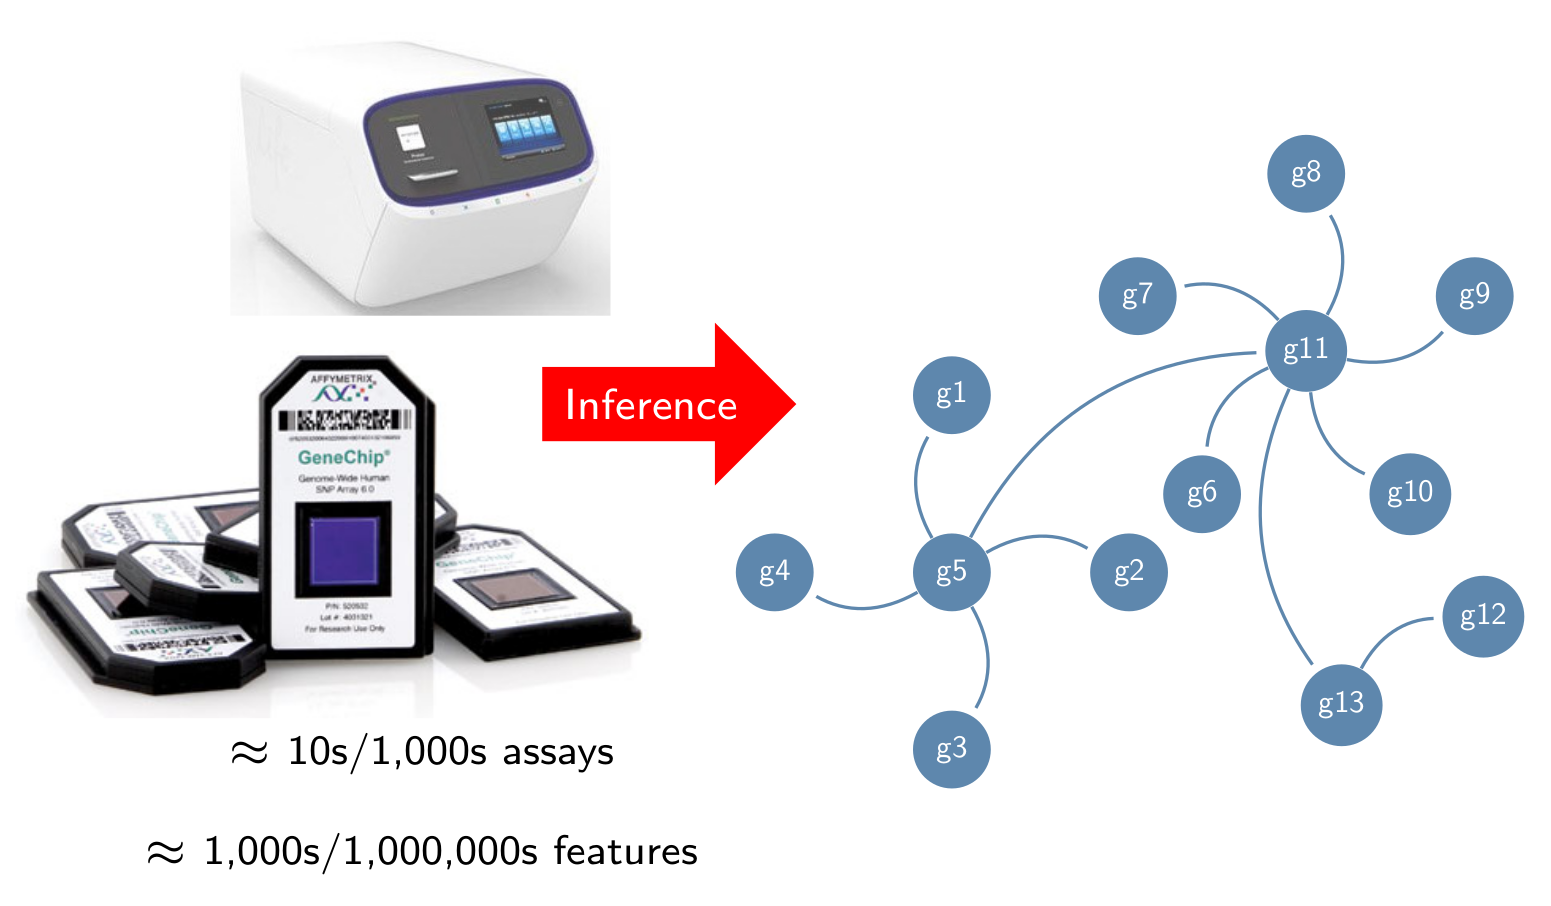
\includegraphics[width=.65\textwidth]{\fignet/Chi18-JC2BIM-p7}
  $$

  \pause
  That is, 
  \begin{itemize}
    \item go from gene expression $Y$ measurements to a gene network $G$ \\
      (replace 'gene' with 'microbe', 'neurone', ...), 
    \item i.e. go from information collected on the nodes to connexions between them.
  \end{itemize}

}

%-------------------------------------------------------------------------------
\frame{ \frametitle{Statistical model}

  \paragraph{Observed data.} The expression vector for sample $i$:
  $$
  y_i = [y_{i1} \dots y_{ij} \dots y_{ip}]
  $$
  is seen as a realisation of a random vector
  $$
  Y_i = [Y_{i1} \dots Y_{ij} \dots Y_{ip}]
  $$

  \bigskip \pause
  \paragraph{Statistical model.} 
  $$
  Y_i \sim p
  $$

  \bigskip \bigskip \pause
  \paragraph{Where is the network (graph)?} \\ ~
  \begin{itemize}
    \item The graph $G$ has to be encoded in the distribution $p$ in some way \\ ~
    \item \emphase{Graphical models} establish a formal connexion between $p$ and $G$
  \end{itemize}

  
}

%-------------------------------------------------------------------------------
%-------------------------------------------------------------------------------
\subsection{Graphical models}
%-------------------------------------------------------------------------------
\frame{\frametitle{Graphical models} 

  \bigskip
  \paragraph{'Interaction':} 
  need for a probabilistic / statistical counterpart for this concept

  \bigskip 
  \paragraph{Translation:} 
  $$
  \text{interactions} 
  := 
  \text{dependency structure of a set of random variables}
  $$

  \pause\bigskip
  \begin{tabular}{lll}
    \paragraph{Graphical models:} &
    \paragraph{Directed models.} ~ &
    \paragraph{Undirected models.} ~ \\
    \begin{tabular}{p{0.3\textwidth}} A generic \\ framework \\ \refer{Lau96,WaJ08}
    \end{tabular}
    & 
    \begin{tabular}{p{0.3\textwidth}}   \begin{tikzpicture}
    \node[observed] (a) at (.5*\edgeunit, 2.75*\edgeunit) {$A$};
  \node[observed] (b) at (0*\edgeunit, 2*\edgeunit) {$B$};
  \node[observed] (c) at (1*\edgeunit, 2*\edgeunit) {$C$};
  \node[observed] (d) at (0.5*\edgeunit, 1*\edgeunit) {$D$};
  \node[observed] (e) at (0*\edgeunit, 0*\edgeunit) {$E$};
  \node[observed] (f) at (1*\edgeunit, 0*\edgeunit) {$F$};

  
  \draw[arrow] (a) to (b);  \draw[arrow] (a) to (c);
  \draw[arrow] (b) to (d);  \draw[arrowbendleft] (b) to (f);
  \draw[arrow] (c) to (d);  \draw[arrow] (d) to (e);
  \draw[arrow] (d) to (f);  
  \end{tikzpicture}
 \end{tabular}
    & 
    \begin{tabular}{p{0.3\textwidth}}   \begin{tikzpicture}
  %   \node[observed] (a) at (0.75*\edgeunit, 1.5*\edgeunit) {$A$};
%   \node[observed] (b) at (0*\edgeunit, 0.75*\edgeunit) {$B$};
%   \node[observed] (c) at (0.75*\edgeunit, 0*\edgeunit) {$C$};
%   \node[observed] (d) at (1.5*\edgeunit, 0.75*\edgeunit) {$D$};
%   \node[observed] (e) at (2.25*\edgeunit, 0*\edgeunit) {$E$};
%   \node[observed] (f) at (3*\edgeunit, 0.75*\edgeunit) {$F$};
%   \node[observed] (g) at (2.25*\edgeunit, 1.5*\edgeunit) {$G$};

  \node[observed] (a) at (.5*\edgeunit, 3*\edgeunit) {$A$};
  \node[observed] (b) at (0*\edgeunit, 2.25*\edgeunit) {$B$};
  \node[observed] (c) at (1*\edgeunit, 2.25*\edgeunit) {$C$};
  \node[observed] (d) at (0.5*\edgeunit, 1.5*\edgeunit) {$D$};
  \node[observed] (e) at (0*\edgeunit, .75*\edgeunit) {$E$};
  \node[observed] (f) at (1*\edgeunit, .75*\edgeunit) {$F$};
  \node[observed] (g) at (.5*\edgeunit, 0*\edgeunit) {$G$};

  
  \draw[edge] (a) to (b);  \draw[edge] (a) to (c);  \draw[edge] (a) to (d);
  \draw[edge] (b) to (c);  \draw[edge] (b) to (d);  \draw[edge] (c) to (d);
  \draw[edge] (d) to (e);  \draw[edge] (d) to (f);  \draw[edge] (e) to (f);
  \draw[edge] (f) to (g);  
  \end{tikzpicture}

 \end{tabular}
    \end{tabular}
  }

%==================================================================
\frame{\frametitle{Undirected graphs = Markov random fields}

  \paragraph{Definition.} Let $G$ be an {\sl undirected graph}, the distribution $p$ is said faithful to $G$ if
  $$
  p(y_1, \dots y_n) \propto \prod_{C \in \Ccal(G)} \psi_C(y_C).
  $$
  where $\Ccal(G)$ is the set of (maximal) cliques of $G$

  \bigskip \bigskip \pause
  \begin{tabular}{cc}
    \begin{tabular}{c}
    $  \begin{tikzpicture}
  %   \node[observed] (a) at (0.75*\edgeunit, 1.5*\edgeunit) {$A$};
%   \node[observed] (b) at (0*\edgeunit, 0.75*\edgeunit) {$B$};
%   \node[observed] (c) at (0.75*\edgeunit, 0*\edgeunit) {$C$};
%   \node[observed] (d) at (1.5*\edgeunit, 0.75*\edgeunit) {$D$};
%   \node[observed] (e) at (2.25*\edgeunit, 0*\edgeunit) {$E$};
%   \node[observed] (f) at (3*\edgeunit, 0.75*\edgeunit) {$F$};
%   \node[observed] (g) at (2.25*\edgeunit, 1.5*\edgeunit) {$G$};

  \node[observed] (a) at (.5*\edgeunit, 3*\edgeunit) {$A$};
  \node[observed] (b) at (0*\edgeunit, 2.25*\edgeunit) {$B$};
  \node[observed] (c) at (1*\edgeunit, 2.25*\edgeunit) {$C$};
  \node[observed] (d) at (0.5*\edgeunit, 1.5*\edgeunit) {$D$};
  \node[observed] (e) at (0*\edgeunit, .75*\edgeunit) {$E$};
  \node[observed] (f) at (1*\edgeunit, .75*\edgeunit) {$F$};
  \node[observed] (g) at (.5*\edgeunit, 0*\edgeunit) {$G$};

  
  \draw[edge] (a) to (b);  \draw[edge] (a) to (c);  \draw[edge] (a) to (d);
  \draw[edge] (b) to (c);  \draw[edge] (b) to (d);  \draw[edge] (c) to (d);
  \draw[edge] (d) to (e);  \draw[edge] (d) to (f);  \draw[edge] (e) to (f);
  \draw[edge] (f) to (g);  
  \end{tikzpicture}

$
    \end{tabular}
    &
    \begin{tabular}{p{.7\textwidth}}
      \begin{eqnarray*}
%         p(a, \dots g) & \propto 
%         & \psi_1(a, b, c) \; \psi_2(a, b, d) \; \psi_3(a, c, d) \; \psi_4(b, c, d) \\
%         & & \psi_5(d, e, f) \; \psi_6(f, g) \\\pause
%       \text{but also} \qquad \\
        p(a, \dots g) & \propto 
        & \psi_1(a, b, c, d) \\
        & & \psi_2(d, e, f) \; \psi_3(f, g) 
      \end{eqnarray*}
%       \ra Only consider \emphase{maximal} cliques
    \end{tabular}
  \end{tabular}
}

%====================================================================
\frame{\frametitle{Conditional independence}

  \paragraph{Property.} If $p(y) > 0$, 
  $$
  \text{separation} \qquad \Leftrightarrow \qquad \text{conditional independence}
  $$

  \bigskip \pause
  \begin{tabular}{ccc}
    \hspace{.2\textwidth} 
    &
    \begin{tabular}{c}
    $  \begin{tikzpicture}
  %   \node[observed] (a) at (0.75*\edgeunit, 1.5*\edgeunit) {$A$};
%   \node[observed] (b) at (0*\edgeunit, 0.75*\edgeunit) {$B$};
%   \node[observed] (c) at (0.75*\edgeunit, 0*\edgeunit) {$C$};
%   \node[observed] (d) at (1.5*\edgeunit, 0.75*\edgeunit) {$D$};
%   \node[observed] (e) at (2.25*\edgeunit, 0*\edgeunit) {$E$};
%   \node[observed] (f) at (3*\edgeunit, 0.75*\edgeunit) {$F$};
%   \node[observed] (g) at (2.25*\edgeunit, 1.5*\edgeunit) {$G$};

  \node[observed] (a) at (.5*\edgeunit, 3*\edgeunit) {$A$};
  \node[observed] (b) at (0*\edgeunit, 2.25*\edgeunit) {$B$};
  \node[observed] (c) at (1*\edgeunit, 2.25*\edgeunit) {$C$};
  \node[observed] (d) at (0.5*\edgeunit, 1.5*\edgeunit) {$D$};
  \node[observed] (e) at (0*\edgeunit, .75*\edgeunit) {$E$};
  \node[observed] (f) at (1*\edgeunit, .75*\edgeunit) {$F$};
  \node[observed] (g) at (.5*\edgeunit, 0*\edgeunit) {$G$};

  
  \draw[edge] (a) to (b);  \draw[edge] (a) to (c);  \draw[edge] (a) to (d);
  \draw[edge] (b) to (c);  \draw[edge] (b) to (d);  \draw[edge] (c) to (d);
  \draw[edge] (d) to (e);  \draw[edge] (d) to (f);  \draw[edge] (e) to (f);
  \draw[edge] (f) to (g);  
  \end{tikzpicture}

$
    \end{tabular}
    &
    \begin{tabular}{p{.7\textwidth}}
    \begin{itemize}
     \item $A \not\independent B$ \\ ~
     \item $A \not\independent D \mid B$ \\ ~
     \item $A \not\independent D \mid \{B, C\}$ \\ ~
     \item $\{A, B, C\} \independent \{E, F, G\} \mid D$ \\ ~
     \item $\{B, C\} \independent \{E, F\} \mid D$ \\ ~
    \end{itemize}
    \end{tabular}
  \end{tabular}

  \bigskip
  \ra Inferring $G$ = Inferring conditional {\sl dependences} = 'direct interactions'
}
  
%==================================================================
\frame{\frametitle{Recovering $G$ from $Y$: Not an easy task}

  \paragraph{A huge search space:}
  $$
  \includegraphics[trim=50 50 0 75, height=.5\textheight, clip]{\fignet/NbGraphs2}
  $$
  Number of \textcolor{darkgreen}{undirected graphs} ($2^{p(p-1)/2}$), \textcolor{red}{directed acyclic graphs} (no close form), \textcolor{blue}{spanning trees} ($p^{p-2}$)
  
  \bigskip \pause
  \paragraph{A common assumption:} 
  \begin{align*}
  \text{$G$ is sparse} \qquad 
  & \Leftrightarrow \qquad \text{Each node has few neighbors}   \\
  & \Leftrightarrow \qquad \text{Each gene directly interacts with few other genes} 
  \end{align*}
}

%==================================================================
\subsection*{Gaussian graphical models (GGM)}
%==================================================================

%==================================================================
\frame{\frametitle{Gaussian graphical models (GGM)}

  \paragraph{Gaussian setting.} Suppose that each 'expression' vector $Y_i = (Y_{i1} \dots Y_{ip})$ is Gaussian
  $$
  Y_i \sim \Ncal_p(\mu, \Sigma)
  $$
  \begin{itemize}
   \item $\mu = (p \times 1)$ vector of mean expressions
   \item $\Sigma = (p \times p)$ covariance matrix:
   $$
   \sigma_{jj} = \sigma_j^2 = \Var(Y_{ij}), \qquad
   \sigma_{jk} = \Cov(Y_{ij}, Y_{ik}), \qquad
   \rho_{jk} = \frac{\sigma_{jk}}{\sigma_j \sigma_k}
   $$
  \end{itemize}

  \bigskip \pause
  \paragraph{Property.}
  $$
  \text{null correlation} \quad \Leftrightarrow \qquad
  \text{null covariance} \quad \Leftrightarrow \qquad
  \text{independence} 
  $$
  i.e.
  $$
  \sigma_{jk} = 0 \quad \Leftrightarrow \qquad Y_{ij} \independent Y_{ik} 
  \pause \emphase{\text{ marginally}}
  $$
}

%==================================================================
\frame{\frametitle{Regression point of view}

  \paragraph{Gene-by-gene approach:} Finding the neighbors of a node is equivalent to find its 'parents' in a regression:
  $$
  Y_{ik} = \sum_{j \neq k} \beta_{jk} Y_{ij} + E_{ik}.
  $$
  \ra Requires a testing procedure \refer{VeV09} or a penalization \refer{MeB06} to determine non-zero coefficients

  \bigskip \bigskip \pause
  \paragraph{Remarks.}
  \begin{itemize}
   \item Regression needs reconciliation when $\widehat{\beta}_{jk} = 0$ and $\widehat{\beta}_{jk} \neq 0$ 
   \item \refer{Ver12} provides bounds for the recovery of the list of neighbors: let $d =$ degree of a given node 
   \begin{align*}
    d \log(p/d) & \leq n & & \text{possible recovery} \\
    d \log(p/d) & > n \log n & & \text{impossible recovery}
   \end{align*}
  \end{itemize}
}

%==================================================================
\frame{\frametitle{A nice property of GGM's}

  \begin{tabular}{cc}
    \begin{tabular}{p{.5\textwidth}}
    \hspace{-.15\textwidth}
    \includegraphics[width=.6\textwidth]{\fignet/FigGGM-4nodes}
    \end{tabular}
    & 
    \hspace{-.15\textwidth}
    \begin{overprint}
    \onslide<2>
    \begin{tabular}{p{.5\textwidth}}
	 \paragraph{Graphical model.}
	 $$
	 G = \left[ \begin{array}{cccc}
	 0 & 1 & 1 & \emphase{0} \\
	 1 & 0 & 1 & \emphase{0} \\
	 1 & 1 & 0 & 1 \\
	 \emphase{0} & \emphase{0} & 1 & 0 
	 \end{array} \right]
	 $$
	 \bigskip
	 \begin{itemize}
	  \item Connected \\ ~
	  \item 3 separates 4 from (1, 2)
	 \end{itemize}
    \end{tabular} 
    \onslide<3>
    \begin{tabular}{p{.5\textwidth}}
	 \paragraph{Covariance matrix.}
	 $$
	 \Sigma \propto \left[ \begin{array}{cccc}
	   1 & -.25 & -.41 &  \emphase{.25} \\
	   -.25 &  1 & -.41 &  \emphase{.25} \\
	   -.41 & -.41 &  1 & -.61 \\
	   \emphase{.25} &  \emphase{.25} & -.61 &  1
	   \end{array} \right] 
	 $$
	 \bigskip
	 \begin{itemize}
	  \item No zero because $G$ is Connected
	 \end{itemize}
    \end{tabular} 
    \onslide<4>
    \begin{tabular}{p{.5\textwidth}}
	 \paragraph{Inverse covariance matrix.}
	 $$
	 \Sigma^{-1} \propto \left[ \begin{array}{cccc}
	   1 & .5 & .5 & \emphase{0} \\
	   .5 & 1 & .5 & \emphase{0} \\
	   .5 & .5 & 1 & .5 \\
	   \emphase{0} & \emphase{0} & .5 & 1
	   \end{array} \right] 
	 $$
	 \bigskip
	 \begin{itemize}
	  \item 0's at (1, 4) and (2, 4)\\ ~
	  \item Conditional independence\\ ~
	  \item $\Omega := \Sigma^{-1} =$ \emphase{precision} matrix
	 \end{itemize}
    \end{tabular} 
    \end{overprint}
  \end{tabular}

}

%==================================================================
\frame{\frametitle{More formally}

  \paragraph{If $Y \sim \Ncal(0, \Omega^{-1})$,} then
  \begin{align*}
  p(Y) & \propto \exp\left(-\frac12 \|Y\|^2_\Omega \right)\\
  & = \exp\left(-\frac12 \sum_{j, k} \omega_{jk} Y_j Y_k\right)  
  & & \text{where } \Omega = [\omega_{jk}] \\
  & = \prod_{j, k} \underset{\phi_{jk}(Y_j, Y_k)}{\underbrace{\exp\left(-\frac12 \omega_{jk} Y_j Y_k\right)}}
  \end{align*}

  \bigskip \pause
  \begin{itemize}
   \item The non-zeros of $\Omega$ correspond to the edges of $G$\\ ~
   \item Furthermore:
   $$
   - \omega_{jk} \; \propto \; 
   \Cor\left(Y_j, Y_k \mid Y_{\{j, k\}}\right)
   = \text{ \emphase{'partial'} correlation}
   $$
  \end{itemize}
  
}

%==================================================================
\frame{\frametitle{Inference}

\begin{tabular}{cc}
    \begin{tabular}{p{.5\textwidth}}
    \hspace{-.15\textwidth}
    \includegraphics[width=.6\textwidth]{\fignet/FigGGM-4nodes}
    \end{tabular}
    & 
    \hspace{-.15\textwidth}
    \begin{overprint}
    \onslide<1>
    \begin{tabular}{p{.5\textwidth}}
	 \paragraph{Graphical model.}
	 $$
	 G = \left[ \begin{array}{cccc}
	 0 & 1 & 1 & \emphase{0} \\
	 1 & 0 & 1 & \emphase{0} \\
	 1 & 1 & 0 & 1 \\
	 \emphase{0} & \emphase{0} & 1 & 0 
	 \end{array} \right]
	 $$
    \end{tabular} 
    \onslide<2>
    \begin{tabular}{p{.5\textwidth}}
	 \paragraph{Inverse covariance matrix.}
	 $$
	 \Omega \propto \left[ \begin{array}{cccc}
	   1 & .5 & .5 & \emphase{0} \\
	   .5 & 1 & .5 & \emphase{0} \\
	   .5 & .5 & 1 & .5 \\
	   \emphase{0} & \emphase{0} & .5 & 1
	   \end{array} \right] 
	 $$
	 \bigskip
	 \begin{itemize}
	  \item Same zeros as $G$
	 \end{itemize}
    \end{tabular} 
    \onslide<3>
    \begin{tabular}{p{.5\textwidth}}
	 \paragraph{Estimated inverse covariance matrix.}
	 $$
	 \widehat{\Omega} \propto \left[ \begin{array}{cccc}
	   1 & .48 & .61 & \emphase{.09} \\
	   .48 & 1 & .67 & \emphase{.06} \\
	   .61 & .67 & 1 & .46 \\
	   \emphase{.09} & \emphase{.06} & .46 & 1
	   \end{array} \right] 
	 $$
	 ($n = 100$)
	 \bigskip
	 \begin{itemize}
	  \item No 'true zero' in the estimate\\ ~
	  \item Need to 'force' zeros to appear
	 \end{itemize}
    \end{tabular} 
    \end{overprint}
  \end{tabular}
}

%==================================================================
\frame{\frametitle{Making $\Omega$ sparse}

  \paragraph{Graphical lasso \refer{FHT08}.} Penalized likelihood:
  $$
  \max_{\mu, \Omega} \log p(Y; \mu, \Omega) - \lambda \sum_{j < k} |\omega_{jk}|
  $$
  the '$\ell_1$' penalty ($|\omega_{jk}|$) forces some $\omega_{jk}$ to be zero. \\
  \ra The higher $\lambda$, the sparser $\widehat{G}$ \\
  \ra Again a convex problem \\
  \ra Fast solution (e.g. {\tt huge} R package)
  
  \bigskip \bigskip \pause
  \paragraph{Playing with penalties.}
  \begin{itemize}
   \item Other forms of penalties ($\ell_1$, $\ell_2$, combinations) induces other topologies
   \item Ex.: \refer{ACM09} induce clustered networks.
  \end{itemize}
  
  \bigskip \bigskip \pause
  \paragraph{Alternatives.}
  \begin{itemize}
   \item Mixture of tree-shaped distributions: \refer{MeJ06,Kir07,JFS16,ScR17,MRA19}
   \item ...
  \end{itemize}
}

